To avoid steady state error, it Is necessary to examine PID controller, which stands for proportional integrate derivative controller. In the following sections there will be an explanation of PID controller, and afterwards there will be a section of what have been chosen for this project.  


\section{PID controller} % ???Different Controller
% her skal der skrives om de forskellige kontrollers (p-, pd-, pi-, pid-controller) og vaglet af vores kontroller
\begin{figure}[H]
    \centering
    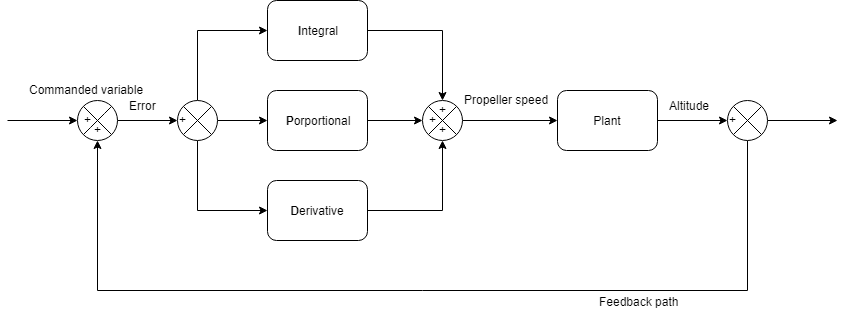
\includegraphics[width=0.9\textwidth]{figures/ch_design/PIDControl.png}
    \caption{Block diagram of a PID control system}
    \label{fig:PID_Controller}
\end{figure}

\section{Design of proportional controller}\label{sec:design_controller}
As it has been decided to use a proportional controller to regulate the system, the proportional gain $K_P$ has to be found. 
